\documentclass{article}
\usepackage[utf8]{vietnam}
\usepackage{pgfplots}
\usepackage{hyperref}
\usepackage{amsmath}
\usepackage{amsfonts}
\usepackage{amssymb}
\usepackage{graphicx}
\usepackage{hyperref}

\title{Bài 1: Năng lượng và chiều dài liên kết /ndt1}
\begin{document}
	\maketitle \emph{\textit{Email: duythe.276051@gmail.com}}
	\section{Vẽ đồ thị và nhận xét}
\textit{\textbf{Tìm hiểu phần mềm Gaussian qua đó hiểu thêm lý thuyết và so sánh với kết quả thực nghiệm:}}\\
\\Sử dụng Gaussian để chạy file chứa tọa độ các nguyên tử của phân tử $ H_2 $ để tính năng lượng toàn phần (Ha) từ 0.05 ($ \mathring{A} $) đến 15 ($ \mathring{A} $) độ dài liên kết. Kết quả thu được số liệu:
\\
\\\url{https://github.com/nguyenthe123/MaterialsScience/}
\newpage
	\subsection{Đồ thị các cơ sở}
	\textit{Các cơ sở: 3-21G, STO-3G, 3-21G, 4-31G, 6-31G và 6-311G.}
\\Đồ thị :
\\
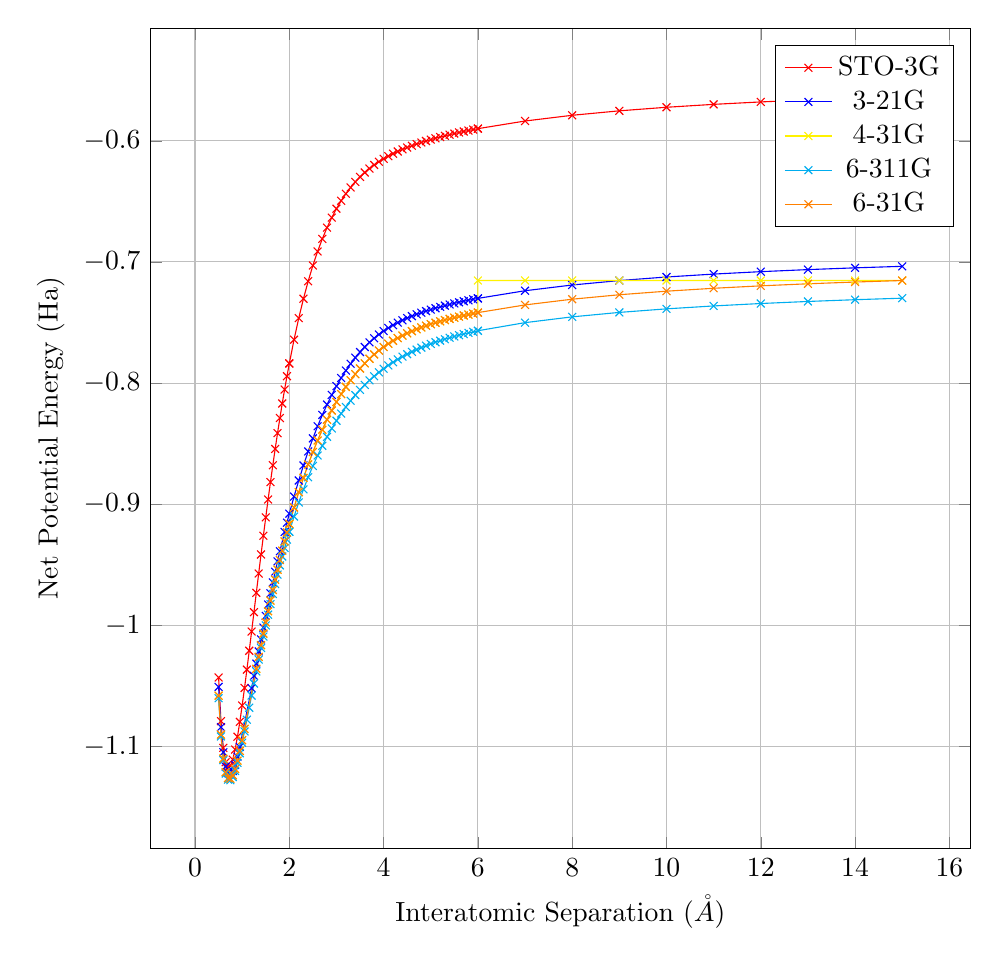
\begin{tikzpicture}
	\begin{axis}[
		height=12cm,
		width=12cm,
		grid=major,
		ylabel=Net Potential Energy (Ha),
		xlabel=Interatomic Separation ($\mathring{A} $)
		]
		\addplot[color=red,mark=x] coordinates {
			(0.5,-1.04299627382)
			(0.55,-1.07905073568)
			(0.6,-1.10112824196)
			(0.65,-1.11299654553)
			(0.7,-1.11734903500)
			(0.75,-1.11615144908)
			(0.8,-1.11085039772)
			(0.85,-1.10251055426)
			(0.9,-1.09191404143)
			(0.95,-1.07963692869)
			(1.0,-1.06610864985)
			(1.05,-1.05165675623)
			(1.1,-1.03653887566)
			(1.15,-1.02096414425)
			(1.2,-1.00510670728)
			(1.25,-0.989113814836)
			(1.3,-0.973110616550)
			(1.35,-0.957203175869)
			(1.4,-0.941480655518)
			(1.45,-0.926017176556)
			(1.5,-0.910873555413)
			(1.55,-0.896098959138)
			(1.6,-0.881732450747)
			(1.65,-0.867804384784)
			(1.7,-0.854337627711)
			(1.75,-0.841348599188)
			(1.8,-0.828848148631)
			(1.85,-0.816842292925)
			(1.9,-0.805332845536)
			(1.95,-0.794317966127)
			(2.0,-0.783792654860)
			(2.0,-0.783792654860)
			(2.1,-0.764177652149)
			(2.2,-0.746401350486)
			(2.3,-0.730353321829)
			(2.4,-0.715910060924)
			(2.5,-0.702943600208)
			(2.6,-0.691327561712)
			(2.7,-0.680940761180)
			(2.8,-0.671668860363)
			(2.9,-0.663404742272)
			(3.0,-0.656048251885)
			(3.1,-0.649505776698)
			(3.2,-0.643689931900)
			(3.3,-0.638519434598)
			(3.4,-0.633919133956)
			(3.5,-0.629820111191)
			(3.6,-0.626159759193)
			(3.7,-0.622881774838)
			(3.8,-0.619936029671)
			(3.9,-0.617278314554)
			(4.0,-0.614869975345)
			(4.1,-0.612677468558)
			(4.2,-0.610671869512)
			(4.3,-0.608828363420)
			(4.4,-0.607125744446)
			(4.5,-0.605545941129)
			(4.6,-0.604073580071)
			(4.7,-0.602695594165)
			(4.8,-0.601400877284)
			(4.9,-0.600179984254)
			(5.0,-0.599024872991)
			(5.1,-0.597928684602)
			(5.2,-0.596885556885)
			(5.3,-0.595890466708)
			(5.4,-0.594939097078)
			(5.5,-0.594027725157)
			(5.6,-0.593153128000)
			(5.7,-0.592312503254)
			(5.8,-0.591503402502)
			(5.9,-0.590723675293)
			(6.0,-0.589971422228)
			(6.0,-0.589971422228)
			(7.0,-0.583659446445)
			(8.0,-0.578934309340)
			(9.0,-0.575259462650)
			(10.0,-0.572319589218)
			(11.0,-0.569914238259)
			(12.0,-0.567909779127)
			(13.0,-0.566213698323)
			(14.0,-0.564759914776)
			(15.0,-0.563499969036)
		};
		\addlegendentry{STO-3G}
		\addplot[color=blue,mark=x] coordinates {
			(0.5,-1.05080141088)
			(0.55,-1.08400623141)
			(0.6,-1.10472133264)
			(0.65,-1.11655417166)
			(0.7,-1.12199495545)
			(0.75,-1.12279503573)
			(0.8,-1.12021281809)
			(0.85,-1.11517234994)
			(0.9,-1.10836349530)
			(0.95,-1.10030503605)
			(1.2,-1.05183854764)
			(1.25,-1.04167191864)
			(1.3,-1.03154819079)
			(1.35,-1.02151086620)
			(1.4,-1.01159327689)
			(1.45,-1.00182166356)
			(1.5,-0.992217128201)
			(1.55,-0.982796828562)
			(1.6,-0.973574695365)
			(1.65,-0.964561872953)
			(1.7,-0.955767017266)
			(1.75,-0.947196533755)
			(1.8,-0.938854800503)
			(1.9,-0.922866338928)
			(1.95,-0.915220324823)
			(2.0,-0.907804967920)
			(2.1,-0.893656583049)
			(2.2,-0.880396346355)
			(2.3,-0.867993835549)
			(2.4,-0.856416453710)
			(2.5,-0.845631353034)
			(2.6,-0.835606289471)
			(2.7,-0.826309792582)
			(2.8,-0.817710935778)
			(2.9,-0.809778908214)
			(3.0,-0.802482539193)
			(3.1,-0.795789892288)
			(3.2,-0.789668011475)
			(3.3,-0.784082860321)
			(3.4,-0.778999453967)
			(3.5,-0.774382151320)
			(3.6,-0.770195056673)
			(3.7,-0.766402475944)
			(3.8,-0.762969378914)
			(3.9,-0.759861830357)
			(4.0,-0.757047365504)
			(4.1,-0.754495296347)
			(4.2,-0.752176943711)
			(4.3,-0.750065795889)
			(4.4,-0.748137598300)
			(4.5,-0.746370380927)
			(4.6,-0.744744431529)
			(4.7,-0.743242223308)
			(4.8,-0.741848305990)
			(4.9,-0.740549169174)
			(5.0,-0.739333086465)
			(5.1,-0.738189948258)
			(5.2,-0.737111090176)
			(5.3,-0.736089123126)
			(5.4,-0.735117769785)
			(5.5,-0.734191711172)
			(5.6,-0.733306445814)
			(5.7,-0.732458163019)
			(5.8,-0.731643630848)
			(5.9,-0.730860098713)
			(6.0,-0.730105213924)
			(6.0,-0.730075884205)
			(7.0,-0.723761187695)
			(8.0,-0.719037804753)
			(9.0,-0.715364300912)
			(10.0,-0.712425479162)
			(11.0,-0.710020974209)
			(12.0,-0.708017210090)
			(13.0,-0.706321710244)
			(14.0,-0.704868419332)
			(15.0,-0.703608896570)
		};
		\addlegendentry{3-21G}
		\addplot[color=yellow,mark=x] coordinates {
			(0.5,-1.05802481639)
			(0.55,-1.09016083624)
			(0.6,-1.11003089435)
			(0.65,-1.12119781550)
			(0.7,-1.12612315793)
			(0.75,-1.12654503067)
			(0.8,-1.12371293170)
			(0.85,-1.11853709749)
			(0.9,-1.11168636959)
			(0.95,-1.10365470240)
			(1.0,-1.09480795913)
			(1.05,-1.08541767061)
			(1.3,-1.03582610656)
			(1.35,-1.02600343809)
			(1.4,-1.01632567123)
			(1.45,-1.00681757676)
			(1.5,-0.997497298461)
			(1.55,-0.988378083183)
			(1.6,-0.979469552902)
			(1.65,-0.970778621807)
			(1.7,-0.962310143804)
			(1.75,-0.954067361056)
			(1.8,-0.946052210918)
			(1.85,-0.938265536477)
			(1.9,-0.930707235066)
			(1.95,-0.923376369669)
			(2.0,-0.916271260360)
			(2.0,-0.916271260360)
			(2.1,-0.902728366902)
			(2.2,-0.890053331916)
			(2.3,-0.878214161730)
			(2.4,-0.867174533761)
			(2.5,-0.856895961994)
			(2.6,-0.847339505736)
			(2.7,-0.838466938641)
			(2.8,-0.830241398147)
			(2.9,-0.822627607326)
			(3.0,-0.815591795582)
			(3.1,-0.809101448569)
			(3.2,-0.803125001285)
			(3.3,-0.797631560204)
			(3.4,-0.792590707768)
			(3.5,-0.787972411654)
			(3.6,-0.783747036336)
			(3.7,-0.779885437995)
			(3.8,-0.776359115999)
			(3.9,-0.773140393259)
			(4.0,-0.770202601597)
			(4.1,-0.767520254121)
			(4.2,-0.765069192878)
			(4.3,-0.762826705404)
			(4.4,-0.760771607854)
			(4.5,-0.758884295125)
			(4.6,-0.757146760048)
			(4.7,-0.755542584630)
			(4.8,-0.754056906786)
			(4.9,-0.752676366160)
			(5.0,-0.751389032741)
			(5.1,-0.750184321904)
			(5.2,-0.749052899480)
			(5.3,-0.747986580265)
			(5.4,-0.746978223187)
			(5.5,-0.746021626008)
			(5.6,-0.745111422095)
			(5.7,-0.744242981354)
			(5.8,-0.743412316973)
			(5.9,-0.742615999146)
			(6.0,-0.741851076566)
			(6.0,-0.715322618404)
			(7.0,-0.715322618404)
			(8.0,-0.715322618404)
			(9.0,-0.715322618404)
			(10.0,-0.715322618404)
			(11.0,-0.715322618404)
			(12.0,-0.715322618404)
			(13.0,-0.715322618404)
			(14.0,-0.715322618404)
			(15.0,-0.715322618404)
		};
		\addlegendentry{4-31G}
			\addplot[color=cyan,mark=x] coordinates {
			(0.5,-1.06010223366)
			(0.55,-1.09169821734)
			(0.6,-1.11127760287)
			(0.65,-1.12233170442)
			(0.7,-1.12727489745)
			(0.75,-1.12780518536)
			(0.8,-1.12513525755)
			(0.85,-1.12014250611)
			(0.9,-1.11346928728)
			(0.95,-1.10559108242)
			(1.0,-1.09686353674)
			(1.05,-1.08755535849)
			(1.1,-1.07787155769)
			(1.15,-1.06796995062)
			(1.2,-1.05797290801)
			(1.25,-1.04797573444)
			(1.3,-1.03805267789)
			(1.35,-1.02826129389)
			(1.4,-1.01864568455)
			(1.45,-1.00923897811)
			(1.5,-1.00006529739)
			(1.55,-0.991141379352)
			(1.6,-0.982477945680)
			(1.65,-0.974080882504)
			(1.7,-0.965952260352)
			(1.75,-0.958091210214)
			(1.8,-0.950494664444)
			(1.85,-0.943157969621)
			(1.9,-0.936075379618)
			(1.95,-0.929240440154)
			(2.0,-0.922646278291)
			(2.0,-0.922646278291)
			(2.1,-0.910151897257)
			(2.2,-0.898535372421)
			(2.3,-0.887741162515)
			(2.4,-0.877716077158)
			(2.5,-0.868409570518)
			(2.6,-0.859773777250)
			(2.7,-0.851763468297)
			(2.8,-0.844335971270)
			(2.9,-0.837451063971)
			(3.0,-0.831070850291)
			(3.1,-0.825159632744)
			(3.2,-0.819683795107)
			(3.3,-0.814611702812)
			(3.4,-0.809913621755)
			(3.5,-0.805561650996)
			(3.6,-0.801529662426)
			(3.7,-0.797793240772)
			(3.8,-0.794329619078)
			(3.9,-0.791117607346)
			(4.0,-0.788137514258)
			(4.1,-0.785371063690)
			(4.2,-0.782801308585)
			(4.3,-0.780412545058)
			(4.4,-0.778190229185)
			(4.5,-0.776120898317)
			(4.6,-0.774192097925)
			(4.7,-0.772392314282)
			(4.8,-0.770710912695)
			(4.9,-0.769138080654)
			(5.0,-0.767664775149)
			(5.1,-0.766282673352)
			(5.2,-0.764984126064)
			(5.3,-0.763762113428)
			(5.4,-0.762610202440)
			(5.5,-0.761522507110)
			(5.6,-0.760493648706)
			(5.7,-0.759518719435)
			(5.8,-0.758593247076)
			(5.9,-0.757713161601)
			(6.0,-0.756874763635)
			(6.0,-0.756786476523)
			(7.0,-0.750101607191)
			(8.0,-0.745329208498)
			(9.0,-0.741654480286)
			(10.0,-0.738718261258)
			(11.0,-0.736316066776)
			(12.0,-0.734314203162)
			(13.0,-0.732620286035)
			(14.0,-0.731168331901)
			(15.0,-0.729909953858)
		};
		\addlegendentry{6-311G}
		\addplot[color=orange,mark=x] coordinates {
			(0.5,-1.05802481639)
			(0.55,-1.09016083624)
			(0.6,-1.11003089435)
			(0.65,-1.12119781550)
			(0.7,-1.12612315793)
			(0.75,-1.12654503067)
			(0.8,-1.12371293170)
			(0.85,-1.11853709749)
			(0.9,-1.11168636959)
			(0.95,-1.10365470240)
			(1.0,-1.09480795913)
			(1.05,-1.08541767061)
			(1.3,-1.03582610656)
			(1.35,-1.02600343809)
			(1.4,-1.01632567123)
			(1.45,-1.00681757676)
			(1.5,-0.997497298461)
			(1.55,-0.988378083183)
			(1.6,-0.979469552902)
			(1.65,-0.970778621807)
			(1.7,-0.962310143804)
			(1.75,-0.954067361056)
			(1.8,-0.946052210918)
			(1.85,-0.938265536477)
			(1.9,-0.930707235066)
			(1.95,-0.923376369669)
			(2.0,-0.916271260360)
			(2.1,-0.902728366902)
			(2.2,-0.890053331916)
			(2.3,-0.878214161730)
			(2.4,-0.867174533761)
			(2.5,-0.856895961994)
			(2.6,-0.847339505736)
			(2.7,-0.838466938641)
			(2.8,-0.830241398147)
			(2.9,-0.822627607326)
			(3.0,-0.815591795582)
			(3.1,-0.809101448569)
			(3.2,-0.803125001285)
			(3.3,-0.797631560204)
			(3.4,-0.792590707768)
			(3.5,-0.787972411654)
			(3.6,-0.783747036336)
			(3.7,-0.779885437995)
			(3.8,-0.776359115999)
			(3.9,-0.773140393259)
			(4.0,-0.770202601597)
			(4.1,-0.767520254121)
			(4.2,-0.765069192878)
			(4.3,-0.762826705404)
			(4.4,-0.760771607854)
			(4.5,-0.758884295125)
			(4.6,-0.757146760048)
			(4.7,-0.755542584630)
			(4.8,-0.754056906786)
			(4.9,-0.752676366160)
			(5.0,-0.751389032741)
			(5.1,-0.750184321904)
			(5.2,-0.749052899480)
			(5.3,-0.747986580265)
			(5.4,-0.746978223187)
			(5.5,-0.746021626008)
			(5.6,-0.745111422095)
			(5.7,-0.744242981354)
			(5.8,-0.743412316973)
			(5.9,-0.742615999146)
			(6.0,-0.741851076566)
			(6.0,-0.741819555402)
			(7.0,-0.735475009467)
			(8.0,-0.730750651431)
			(9.0,-0.727077350730)
			(10.0,-0.724138705667)
			(11.0,-0.721734341136)
			(12.0,-0.719730691028)
			(13.0,-0.718035285483)
			(14.0,-0.716582073744)
			(15.0,-0.715322618404)
		};
		\addlegendentry{6-31G}
	\end{axis}
\end{tikzpicture}
	\subsection{Nhận xét đồ thị}
\begin{enumerate}
	\item Đồ thị năng lượng toàn phần này phù hợp với lý thuyết về năng lượng tương tác giữa 2 nguyên tử.
	\item Với phiếm hàm RHF - Cơ sở STO-3G sử dụng 1 AO cho mỗi nguyên tử Hidro nên 2 MO được tính còn 3-21G sử dụng 2 AO cho mỗi nguyên tử nên 4 MO được tính tương tự cơ sở 6-311G, 3 AO cho mỗi nguyên tử Hidro nên 6 AO được tính, tốc độ hội tụ chậm hơn so với cơ sở STO-3G song chính xác hơn. Tương tự với 3 cơ sở còn lại kết luận \textbf{cơ sở 6-311G cho kết quả chính xác hơn.} 
	\item Các cơ sở đều cho kết quả gần như nhau (tại khoảng 0.75 Angstrom đều là cực tiểu của năng lượng), sát với kết quả thực nghiệm, trong đó, ví dụ:\\
	\begin{itemize}
		\item Năng lượng toàn phần cực tiểu: -1.12780518536 Ha tại 0.75 Angstrom (cho cơ sở 6-311G) còn thực nghiệm là tại 0.741 Angstrom là -1.164094083 Ha ).
		\item 	Khoảng cách: Đồ thị chỉ ra \textbf{năng lượng cực tiểu năng lượng tại $ r_0 $ 0.75 Angstrom còn thực nghiệm 0.741 Angstrom} , kết luận phù hợp.
	\end{itemize}
\end{enumerate}
Bảng số liệu tóm tắt kết quả  $ r_0 (\mathring{A})$ và Net Energy(Ha) :\\
\begin{center}
	\begin{tabular}{|c|c|c|}
		\hline
		STO-3G & 0.70 & -1.11734903500 \\
		\hline
		3-21G & 0.75 & -1.12279503573 \\
		\hline
		4-31G & 0.75 & -1.12654503067 \\
		\hline
		6-311G & 0.75 & -1.12780518536 \\
		\hline
		6-31G & 0.75 & -1.12654503067 \\
		\hline
		Exp & 0.741 & -1.164094083 \\
		\hline
	\end{tabular}
\end{center}

\newpage
\subsection{Thay đổi phiếm hàm}
\textit{\textbf{Sử dụng cơ sở STO-3G (thử dùng thay vì 6-311G), thay đổi phiếm hàm RHF bằng LDA (SVWN), GGA (BLYP) và hybrid (B3LY P): }}\\
\\ \textbf{Số liệu:}\\
\\\url{https://github.com/nguyenthe123/MaterialsScience/}\\
\\\textbf{Đồ thị khi thay các phiếm hàm RHF, LDA (SVWN), GGA (BLYP) và hybrid (B3LY P):}\\\\
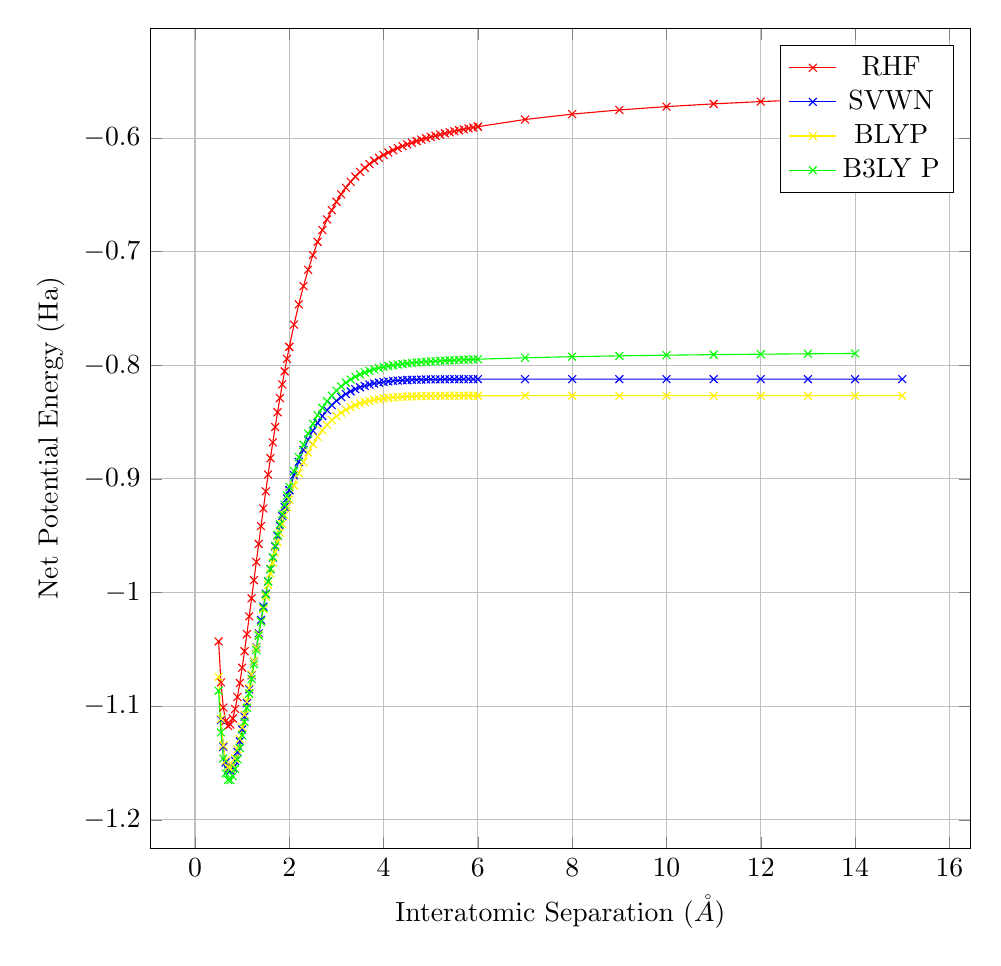
\begin{tikzpicture}
	\begin{axis}[
		height=12cm,
		width=12cm,
		grid=major,
		ylabel=Net Potential Energy (Ha),
		xlabel=Interatomic Separation ($\mathring{A} $)
		]
		\addplot[color=red,mark=x] coordinates {
			(0.5,-1.04299627382)
			(0.55,-1.07905073568)
			(0.6,-1.10112824196)
			(0.65,-1.11299654553)
			(0.7,-1.11734903500)
			(0.75,-1.11615144908)
			(0.8,-1.11085039772)
			(0.85,-1.10251055426)
			(0.9,-1.09191404143)
			(0.95,-1.07963692869)
			(1.0,-1.06610864985)
			(1.05,-1.05165675623)
			(1.1,-1.03653887566)
			(1.15,-1.02096414425)
			(1.2,-1.00510670728)
			(1.25,-0.989113814836)
			(1.3,-0.973110616550)
			(1.35,-0.957203175869)
			(1.4,-0.941480655518)
			(1.45,-0.926017176556)
			(1.5,-0.910873555413)
			(1.55,-0.896098959138)
			(1.6,-0.881732450747)
			(1.65,-0.867804384784)
			(1.7,-0.854337627711)
			(1.75,-0.841348599188)
			(1.8,-0.828848148631)
			(1.85,-0.816842292925)
			(1.9,-0.805332845536)
			(1.95,-0.794317966127)
			(2.0,-0.783792654860)
			(2.0,-0.783792654860)
			(2.1,-0.764177652149)
			(2.2,-0.746401350486)
			(2.3,-0.730353321829)
			(2.4,-0.715910060924)
			(2.5,-0.702943600208)
			(2.6,-0.691327561712)
			(2.7,-0.680940761180)
			(2.8,-0.671668860363)
			(2.9,-0.663404742272)
			(3.0,-0.656048251885)
			(3.1,-0.649505776698)
			(3.2,-0.643689931900)
			(3.3,-0.638519434598)
			(3.4,-0.633919133956)
			(3.5,-0.629820111191)
			(3.6,-0.626159759193)
			(3.7,-0.622881774838)
			(3.8,-0.619936029671)
			(3.9,-0.617278314554)
			(4.0,-0.614869975345)
			(4.1,-0.612677468558)
			(4.2,-0.610671869512)
			(4.3,-0.608828363420)
			(4.4,-0.607125744446)
			(4.5,-0.605545941129)
			(4.6,-0.604073580071)
			(4.7,-0.602695594165)
			(4.8,-0.601400877284)
			(4.9,-0.600179984254)
			(5.0,-0.599024872991)
			(5.1,-0.597928684602)
			(5.2,-0.596885556885)
			(5.3,-0.595890466708)
			(5.4,-0.594939097078)
			(5.5,-0.594027725157)
			(5.6,-0.593153128000)
			(5.7,-0.592312503254)
			(5.8,-0.591503402502)
			(5.9,-0.590723675293)
			(6.0,-0.589971422228)
			(6.0,-0.589971422228)
			(7.0,-0.583659446445)
			(8.0,-0.578934309340)
			(9.0,-0.575259462650)
			(10.0,-0.572319589218)
			(11.0,-0.569914238259)
			(12.0,-0.567909779127)
			(13.0,-0.566213698323)
			(14.0,-0.564759914776)
			(15.0,-0.563499969036)
		};
		\addlegendentry{RHF}
		\addplot[color=blue,mark=x] coordinates {
			(0.55,-1.11197871500)
			(0.6,-1.13570418050)
			(0.65,-1.14942366596)
			(0.7,-1.15582107485)
			(0.75,-1.15685286578)
			(0.8,-1.15395723258)
			(0.85,-1.14819133985)
			(0.9,-1.14033031460)
			(0.95,-1.13094313188)
			(1.0,-1.12045141529)
			(1.05,-1.10917368572)
			(1.1,-1.09735701348)
			(1.15,-1.08519840475)
			(1.2,-1.07285838776)
			(1.25,-1.06046943183)
			(1.3,-1.04814106442)
			(1.35,-1.03596335571)
			(1.4,-1.02400944566)
			(1.45,-1.01233786207)
			(1.5,-1.00099447217)
			(1.55,-0.990014487736)
			(1.6,-0.979424111725)
			(1.65,-0.969242053736)
			(1.7,-0.959480874043)
			(1.75,-0.950147896592)
			(1.8,-0.941246152688)
			(1.85,-0.932775058331)
			(1.9,-0.924730842954)
			(1.95,-0.917107122066)
			(2.0,-0.909895302712)
			(2.0,-0.909895302712)
			(2.1,-0.896663539415)
			(2.2,-0.884934440754)
			(2.3,-0.874591618765)
			(2.4,-0.865512437244)
			(2.5,-0.857574774153)
			(2.6,-0.850662097779)
			(2.7,-0.844665729218)
			(2.8,-0.839485984611)
			(2.9,-0.835031965829)
			(3.0,-0.831220639547)
			(3.1,-0.827976194557)
			(3.2,-0.825229020777)
			(3.3,-0.822915315095)
			(3.4,-0.820977057982)
			(3.5,-0.819361622537)
			(3.6,-0.818021638781)
			(3.7,-0.816915237570)
			(3.8,-0.816005669121)
			(3.9,-0.815260736240)
			(4.0,-0.814652808332)
			(4.1,-0.814158570938)
			(4.2,-0.813758153160)
			(4.3,-0.813434652418)
			(4.4,-0.813174122044)
			(4.5,-0.812965180817)
			(4.5,-0.812965180817)
			(4.6,-0.812798266589)
			(4.7,-0.812665289100)
			(4.8,-0.812559678832)
			(4.9,-0.812476251934)
			(5.0,-0.812410768484)
			(5.1,-0.812359589479)
			(5.2,-0.812319673458)
			(5.3,-0.812288658490)
			(5.4,-0.812264761388)
			(5.5,-0.812246545263)
			(5.6,-0.812232750010)
			(5.7,-0.812222296055)
			(5.8,-0.812214361590)
			(5.9,-0.812208379874)
			(6.0,-0.812203951238)
			(7.0,-0.812192814071)
			(8.0,-0.812192501601)
			(9.0,-0.812192499486)
			(10.0,-0.812192490298)
			(11.0,-0.812192464461)
			(12.0,-0.812192451609)
			(13.0,-0.812192466390)
			(14.0,-0.812192462069)
			(15.0,-0.812192462192)
		};
		\addlegendentry{SVWN}
		
		\addplot[color=yellow,mark=x] coordinates {
			(0.5,-1.07421934391)
			(0.55,-1.11115007657)
			(0.6,-1.13441795311)
			(0.65,-1.14777585570)
			(0.7,-1.15389927219)
			(0.75,-1.15473714597)
			(0.8,-1.15172247474)
			(0.85,-1.14590970274)
			(0.9,-1.13807302659)
			(0.95,-1.12878123478)
			(1.0,-1.11845549061)
			(1.05,-1.10741283004)
			(1.1,-1.09589741721)
			(1.15,-1.08410186210)
			(1.2,-1.07218098865)
			(1.25,-1.06026057390)
			(1.3,-1.04844283853)
			(1.35,-1.03681028304)
			(1.4,-1.02542851239)
			(1.45,-1.01434877636)
			(1.5,-1.00361008216)
			(1.55,-0.993241295295)
			(1.6,-0.983262855016)
			(1.65,-0.973688315887)
			(1.7,-0.964525711727)
			(1.75,-0.955778472897)
			(1.8,-0.947446352224)
			(1.85,-0.939526094252)
			(1.9,-0.932011832318)
			(1.95,-0.924895608272)
			(2.0,-0.918167748165)
			(2.1,-0.905831080148)
			(2.2,-0.894899602488)
			(2.3,-0.885260006213)
			(2.4,-0.876795239420)
			(2.5,-0.869390174905)
			(2.6,-0.862935804034)
			(2.7,-0.857331180576)
			(2.8,-0.852483971121)
			(2.9,-0.848310470117)
			(3.0,-0.844734121202)
			(3.1,-0.841685412896)
			(3.2,-0.839100307691)
			(3.3,-0.836919991822)
			(3.4,-0.835091066887)
			(3.5,-0.833564715758)
			(3.6,-0.832296931412)
			(3.7,-0.831248906307)
			(3.8,-0.830386236748)
			(3.9,-0.829678682579)
			(4.0,-0.829100529961)
			(4.1,-0.828629915737)
			(4.2,-0.828247914675)
			(4.3,-0.827938697731)
			(4.4,-0.827689353094)
			(4.5,-0.827489036411)
			(4.6,-0.827328573608)
			(4.7,-0.827200431728)
			(4.8,-0.827098538477)
			(4.9,-0.827017922812)
			(5.0,-0.826954450200)
			(5.1,-0.826904719701)
			(5.2,-0.826865872442)
			(5.3,-0.826835680330)
			(5.4,-0.826812363821)
			(5.5,-0.826794544293)
			(5.6,-0.826781030382)
			(5.7,-0.826770779913)
			(5.8,-0.826763001034)
			(5.9,-0.826757125008)
			(6.0,-0.826752762436)
			(6.0,-0.826752762436)
			(7.0,-0.826741747892)
			(8.0,-0.826741398597)
			(9.0,-0.826741416597)
			(10.0,-0.826741414330)
			(11.0,-0.826741375520)
			(12.0,-0.826741366171)
			(13.0,-0.826741366171)
			(14.0,-0.826741366171)
			(15.0,-0.826741366171)
		};
		\addlegendentry{BLYP}	
		
		\addplot[color=green,mark=x] coordinates {
			(0.5,-1.08634562746)
			(0.55,-1.12307082122)
			(0.6,-1.14605900277)
			(0.65,-1.15906722394)
			(0.7,-1.16477585279)
			(0.75,-1.16513837666)
			(0.8,-1.16159147854)
			(0.85,-1.15519238346)
			(0.9,-1.14671744069)
			(0.95,-1.13673738133)
			(1.0,-1.12567550950)
			(1.05,-1.11385150821)
			(1.1,-1.10151286151)
			(1.15,-1.08885619460)
			(1.2,-1.07604096647)
			(1.25,-1.06319805036)
			(1.3,-1.05043505069)
			(1.35,-1.03783994678)
			(1.4,-1.02548376558)
			(1.45,-1.01342297296)
			(1.5,-1.00170150101)
			(1.55,-0.990352759969)
			(1.6,-0.979401318896)
			(1.65,-0.968864422222)
			(1.7,-0.958753330922)
			(1.75,-0.949074266558)
			(1.8,-0.939829335312)
			(1.85,-0.931017215426)
			(1.9,-0.922633603326)
			(1.95,-0.914671748154)
			(2.0,-0.907122855449)
			(2.1,-0.893220113879)
			(2.2,-0.880825265209)
			(2.3,-0.869824235740)
			(2.4,-0.860097191451)
			(2.5,-0.851524894342)
			(2.6,-0.843993357261)
			(2.7,-0.837396146388)
			(2.8,-0.831635210724)
			(2.9,-0.826620958811)
			(3.0,-0.822271064570)
			(3.1,-0.818510256203)
			(3.2,-0.815269026115)
			(3.3,-0.812483383395)
			(3.4,-0.810094993132)
			(3.5,-0.808050550380)
			(3.6,-0.806301935586)
			(3.7,-0.804806515366)
			(3.8,-0.803526503435)
			(3.9,-0.802428672979)
			(4.0,-0.801484550904)
			(4.1,-0.800669827055)
			(4.2,-0.799963511363)
			(4.3,-0.799347900928)
			(4.4,-0.798808362813)
			(4.5,-0.798332596298)
			(4.6,-0.797910183169)
			(4.7,-0.797532457321)
			(4.8,-0.797192322182)
			(4.9,-0.796883923930)
			(5.0,-0.796602362708)
			(5.1,-0.796343541041)
			(5.2,-0.796103995623)
			(5.3,-0.795880943351)
			(5.4,-0.795672112813)
			(5.5,-0.795475662926)
			(5.6,-0.795289995455)
			(5.7,-0.795113716203)
			(5.8,-0.794945704502)
			(5.9,-0.794785081588)
			(6.0,-0.794631159933)
			(7.0,-0.793360002176)
			(8.0,-0.792414698993)
			(9.0,-0.791679743996)
			(10.0,-0.791091766940)
			(11.0,-0.790610665486)
			(12.0,-0.790209765452)
			(13.0,-0.789870572449)
			(14.0,-0.789579805936)
		};
		\addlegendentry{B3LY P}		
	\end{axis}
\end{tikzpicture}\\
\textbf{Nhận xét đồ thị:}
\begin{itemize}
	\item \textbf{Phiếm hàm B3LYP} cho kết quả gần thực nghiệm nhất, năng lượng cực tiểu gần thực nghiệm nhất tại 0.75 Angstrom , ba phiếm hàm sau không tốt bằng khi xét về năng lượng cực tiểu.
\end{itemize}
Bảng số liệu tóm tắt kết quả: \\
\begin{center}
	\begin{tabular}{|c|c|c|}
		\hline
		RHF & 0.70 & -1.11734903500 \\
		\hline
		SVWN & 0.75 & -1.15685286578 \\
		\hline
		BYLP & 0.75 & -1.15473714597 \\
		\hline
		B3LY P & 0.75 & -1.16513837666 \\
		\hline
		Exp & 0.741 & -1.164094083 \\
		\hline
	\end{tabular}
\end{center}
\begin{itemize}
	\item \textbf{Nhận xét bảng :} Ở đây ta không chạy $ r_0 $ = 0.741 Amstrong nên kết quả sử dụng 0.75 Angstrom khó để nhận xét. Song tạm kết luận phiếm hàm B3LY P cho gần kết quả thực nghiệm nhất.
\end{itemize}
\newpage
	%%%%%%%%%%
\subsection{Số liệu HOMO-LUMO gap}
\textit{\textbf{Chạy Gaussian với tọa độ $ r_0 $ = 0.75 Angstrom với các phiếm hàm cho kết quả HOMO-LUMO gap như sau:}}
\begin{center}
	\begin{tabular}{|c|c|c|c|c|}
		\hline
		& HOMO & LUMO & Gap(Ha) & Gap(eV) \\
		\hline
		B3LY P & -0.435316 & 0.057284 & 0.4926 & 13.4036 \\
		\hline
		RHF & -0.592889 & 0.167280 & 0.7602 & 20.6842 \\
		\hline
		BYLP & -0.382798 & 0.037594 & 0.4204 & 11.4389 \\
		\hline
		SVWN & -0.395792 & 0.026442 & 0.4222 & 11.4890 \\
		\hline
		Exp &  &  & 0.4336 & 11.8 \\
		\hline
	\end{tabular}
\end{center}
\textbf{Nhận xét số liệu:}
\begin{itemize}
	\item \textbf{SVWN và BYLP cho kết quả HOMO-LUMO Gap gần số liệu thực nghiệm nhất.}
\end{itemize}
{\large \textbf{Kết luận sau phần 1 : }}
\begin{enumerate}
	\item Cơ sở 6-311G cho năng lượng cực tiểu tại 0.75 Angstrom gần kết quả thực nghiệm nhất.
	\item Phiếm hàm B3LY P cho kết quả năng lượng cực tiểu gần thực nghiệm nhất.
	\item Phiếm hàm BYLP và SVWN cho kết quả HOMO-LUMO gap gần thực nghiệm nhất.
\end{enumerate}
\newpage
\section{Nhận xét bài báo}
	\textbf{ Comparison of DFT Methods for Molecular Orbital Eigenvalue Calculations} -\textbf{\textit{ Gang Zhang and Charles B. Musgrave*}}.
	\\ 
\end{document}